\documentclass{standalone}
\usepackage{tikz}
\usetikzlibrary{patterns, positioning}
\usepackage[sfdefault]{ClearSans} %% option 'sfdefault' activates Clear Sans as the default text font
\usepackage[T1]{fontenc}

\begin{document}
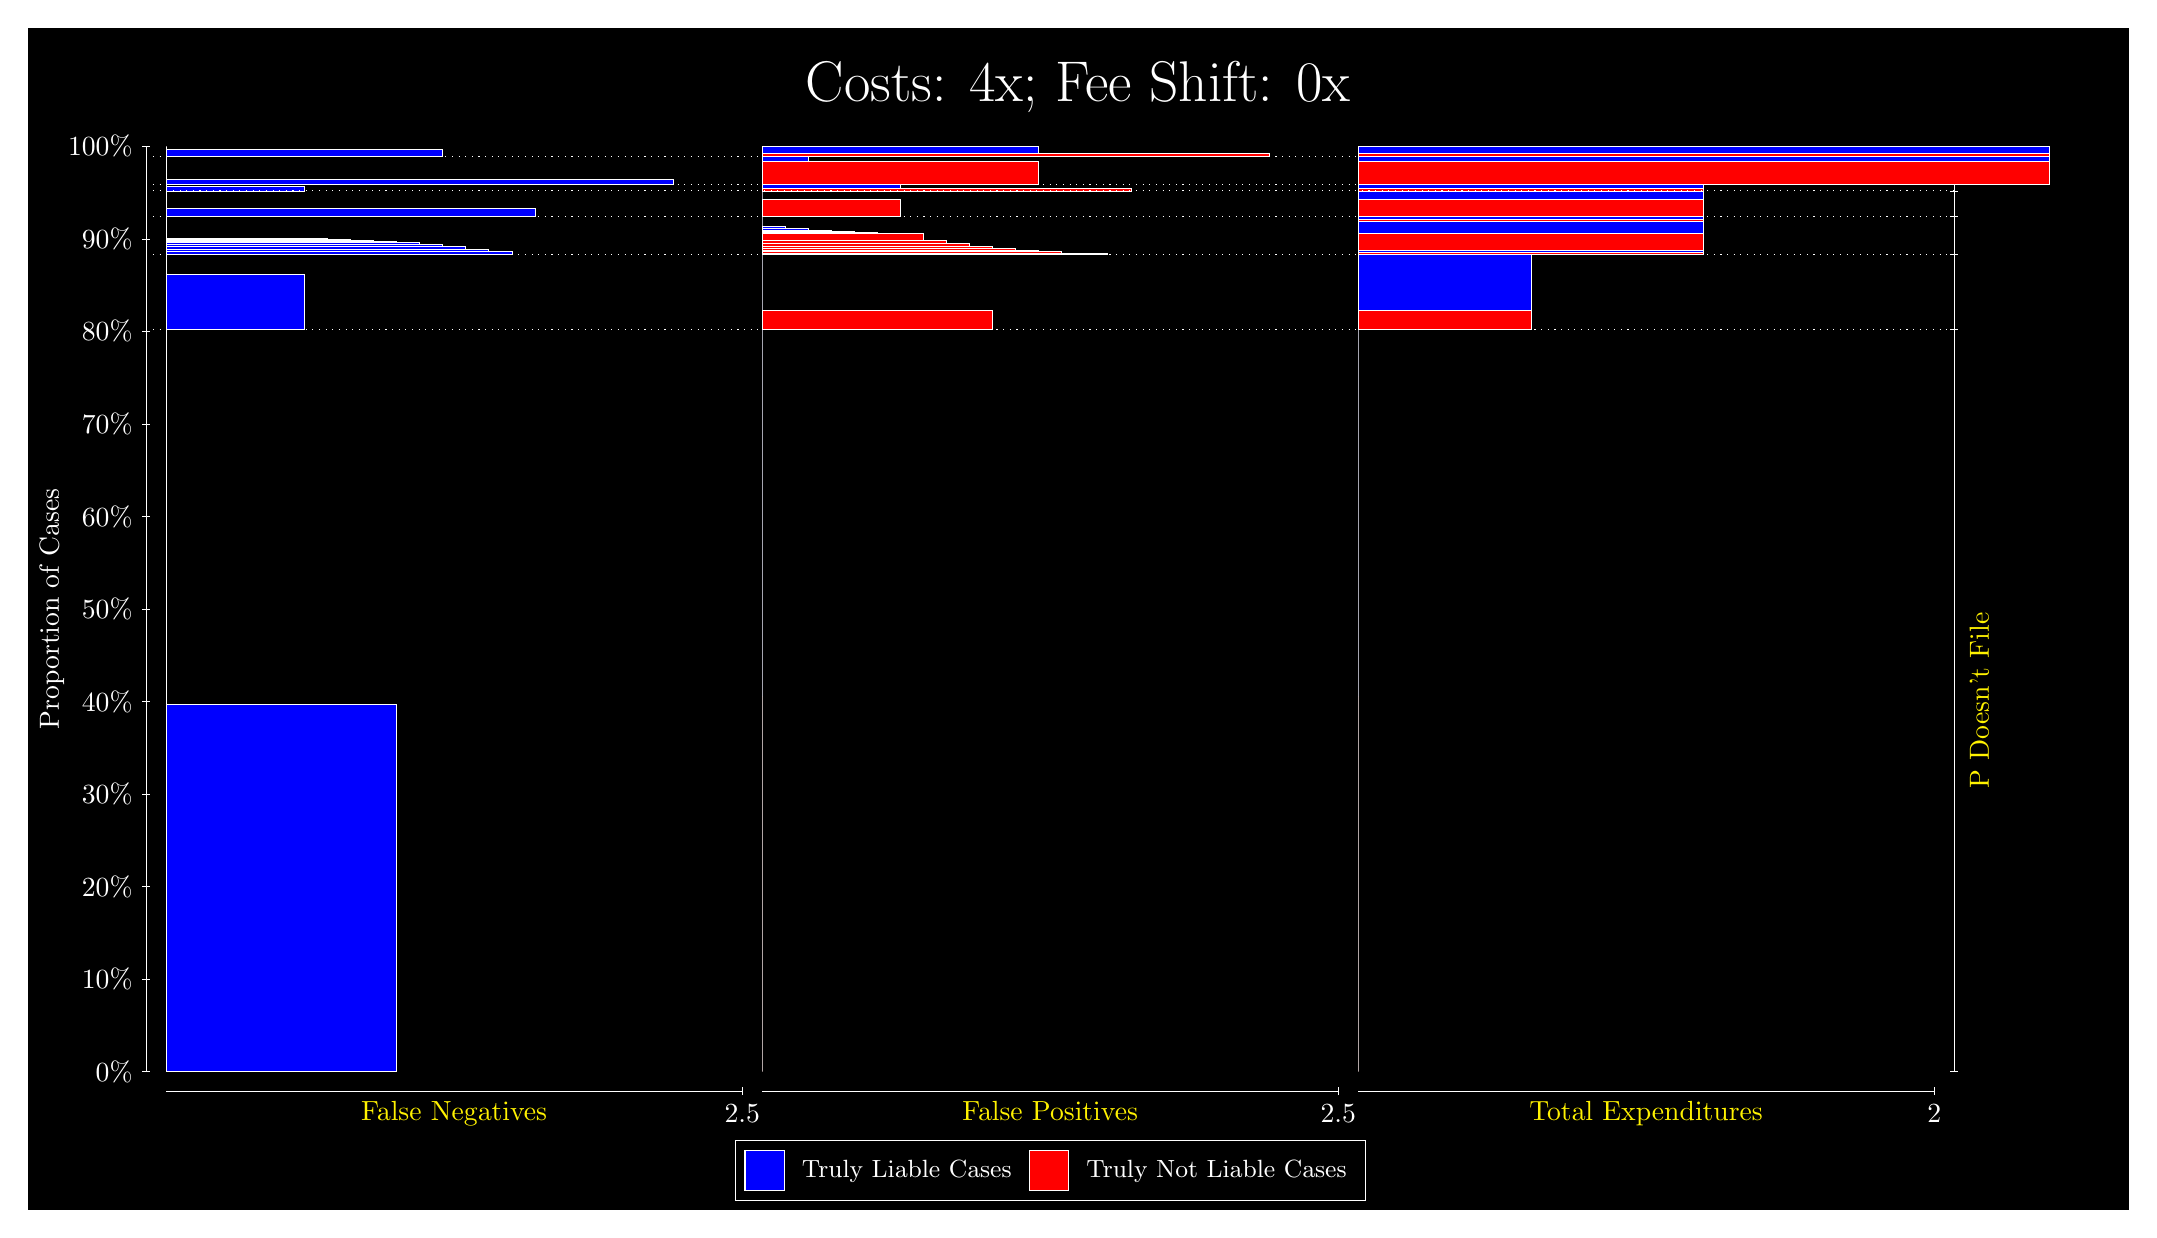
\begin{tikzpicture}
\draw[fill=black] (0,0) rectangle (26.667,15);
\draw[text=white] (0,13.5) rectangle (26.667,15) node[midway] {\huge Costs: 4x; Fee Shift: 0x};
\draw[white, very thin] (1.5,1.75) -- (1.5,13.5);
\node[rotate=90, text=white, anchor=center] at (0.3, 7.625) {Proportion of Cases};
\draw[white, very thin] (1.45,1.75) -- (1.55,1.75);
\node[text=white, anchor=east] at (1.45, 1.75) {0\%};
\draw[white, very thin] (1.45,2.925) -- (1.55,2.925);
\node[text=white, anchor=east] at (1.45, 2.925) {10\%};
\draw[white, very thin] (1.45,4.1) -- (1.55,4.1);
\node[text=white, anchor=east] at (1.45, 4.1) {20\%};
\draw[white, very thin] (1.45,5.275) -- (1.55,5.275);
\node[text=white, anchor=east] at (1.45, 5.275) {30\%};
\draw[white, very thin] (1.45,6.45) -- (1.55,6.45);
\node[text=white, anchor=east] at (1.45, 6.45) {40\%};
\draw[white, very thin] (1.45,7.625) -- (1.55,7.625);
\node[text=white, anchor=east] at (1.45, 7.625) {50\%};
\draw[white, very thin] (1.45,8.8) -- (1.55,8.8);
\node[text=white, anchor=east] at (1.45, 8.8) {60\%};
\draw[white, very thin] (1.45,9.975) -- (1.55,9.975);
\node[text=white, anchor=east] at (1.45, 9.975) {70\%};
\draw[white, very thin] (1.45,11.15) -- (1.55,11.15);
\node[text=white, anchor=east] at (1.45, 11.15) {80\%};
\draw[white, very thin] (1.45,12.325) -- (1.55,12.325);
\node[text=white, anchor=east] at (1.45, 12.325) {90\%};
\draw[white, very thin] (1.45,13.5) -- (1.55,13.5);
\node[text=white, anchor=east] at (1.45, 13.5) {100\%};

\draw[white, very thin] (24.457,1.75) -- (24.457,13.5);
\draw[white, very thin] (24.407,1.75) -- (24.507,1.75);
\node[anchor=west] at (24.407, 1.75) {};
\draw[white, very thin] (24.407,11.175) -- (24.507,11.175);
\node[anchor=west] at (24.407, 11.175) {};
\draw[white, very thin] (24.407,12.126) -- (24.507,12.126);
\node[anchor=west] at (24.407, 12.126) {};
\draw[white, very thin] (24.407,12.606) -- (24.507,12.606);
\node[anchor=west] at (24.407, 12.606) {};
\draw[white, very thin] (24.407,12.935) -- (24.507,12.935);
\node[anchor=west] at (24.407, 12.935) {};
\draw[white, very thin] (24.407,13.02) -- (24.507,13.02);
\node[anchor=west] at (24.407, 13.02) {};
\draw[white, very thin] (24.407,13.372) -- (24.507,13.372);
\node[anchor=west] at (24.407, 13.372) {};
\draw[white, very thin] (24.407,13.5) -- (24.507,13.5);
\node[anchor=west] at (24.407, 13.5) {};

\draw[white, very thin, fill=blue] (1.75,1.75) rectangle (4.6775,6.4087);
\draw[white, very thin, fill=red] (1.75,6.4087) rectangle (1.75,11.175);
\draw[white, very thin, fill=blue] (1.75,11.175) rectangle (3.5065,11.88);
\draw[white, very thin, fill=red] (1.75,11.88) rectangle (1.75,12.126);
\draw[white, very thin, fill=blue] (1.75,12.126) rectangle (6.1413,12.162);
\draw[white, very thin, fill=blue] (1.75,12.162) rectangle (5.8486,12.191);
\draw[white, very thin, fill=blue] (1.75,12.191) rectangle (5.5558,12.232);
\draw[white, very thin, fill=blue] (1.75,12.232) rectangle (5.2631,12.25);
\draw[white, very thin, fill=blue] (1.75,12.25) rectangle (4.9703,12.276);
\draw[white, very thin, fill=blue] (1.75,12.276) rectangle (4.6775,12.294);
\draw[white, very thin, fill=blue] (1.75,12.294) rectangle (4.3848,12.313);
\draw[white, very thin, fill=blue] (1.75,12.313) rectangle (4.092,12.323);
\draw[white, very thin, fill=blue] (1.75,12.323) rectangle (3.7993,12.335);
\draw[white, very thin, fill=red] (1.75,12.335) rectangle (1.75,12.606);
\draw[white, very thin, fill=blue] (1.75,12.606) rectangle (6.4341,12.71);
\draw[white, very thin, fill=red] (1.75,12.71) rectangle (1.75,12.935);
\draw[white, very thin, fill=blue] (1.75,12.935) rectangle (3.5065,12.987);
\draw[white, very thin, fill=red] (1.75,12.987) rectangle (1.75,13.02);
\draw[white, very thin, fill=blue] (1.75,13.02) rectangle (8.1906,13.076);
\draw[white, very thin, fill=red] (1.75,13.076) rectangle (1.75,13.372);
\draw[white, very thin, fill=blue] (1.75,13.372) rectangle (5.2631,13.464);
\draw[white, very thin, fill=red] (1.75,13.464) rectangle (1.75,13.5);
\draw[white, very thin, fill=red] (9.3189,1.75) rectangle (9.3189,6.5166);
\draw[white, very thin, fill=blue] (9.3189,6.5166) rectangle (9.3189,11.175);
\draw[white, very thin, fill=red] (9.3189,11.175) rectangle (12.246,11.422);
\draw[white, very thin, fill=blue] (9.3189,11.422) rectangle (9.3189,12.126);
\draw[white, very thin, fill=red] (9.3189,12.126) rectangle (13.71,12.137);
\draw[white, very thin, fill=red] (9.3189,12.137) rectangle (13.417,12.148);
\draw[white, very thin, fill=red] (9.3189,12.148) rectangle (13.125,12.167);
\draw[white, very thin, fill=red] (9.3189,12.167) rectangle (12.832,12.184);
\draw[white, very thin, fill=red] (9.3189,12.184) rectangle (12.539,12.209);
\draw[white, very thin, fill=red] (9.3189,12.209) rectangle (12.246,12.227);
\draw[white, very thin, fill=red] (9.3189,12.227) rectangle (11.954,12.269);
\draw[white, very thin, fill=red] (9.3189,12.269) rectangle (11.661,12.301);
\draw[white, very thin, fill=red] (9.3189,12.301) rectangle (11.368,12.398);
\draw[white, very thin, fill=blue] (9.3189,12.398) rectangle (10.783,12.409);
\draw[white, very thin, fill=blue] (9.3189,12.409) rectangle (10.49,12.419);
\draw[white, very thin, fill=blue] (9.3189,12.419) rectangle (10.197,12.438);
\draw[white, very thin, fill=blue] (9.3189,12.438) rectangle (9.9044,12.456);
\draw[white, very thin, fill=blue] (9.3189,12.456) rectangle (9.6116,12.482);
\draw[white, very thin, fill=blue] (9.3189,12.482) rectangle (9.3189,12.606);
\draw[white, very thin, fill=red] (9.3189,12.606) rectangle (11.075,12.831);
\draw[white, very thin, fill=blue] (9.3189,12.831) rectangle (9.3189,12.935);
\draw[white, very thin, fill=red] (9.3189,12.935) rectangle (14.003,12.968);
\draw[white, very thin, fill=blue] (9.3189,12.968) rectangle (11.075,13.02);
\draw[white, very thin, fill=red] (9.3189,13.02) rectangle (12.832,13.316);
\draw[white, very thin, fill=blue] (9.3189,13.316) rectangle (9.9044,13.372);
\draw[white, very thin, fill=red] (9.3189,13.372) rectangle (15.759,13.409);
\draw[white, very thin, fill=blue] (9.3189,13.409) rectangle (12.832,13.5);
\draw[white, very thin, fill=red] (16.888,1.75) rectangle (16.888,6.5166);
\draw[white, very thin, fill=blue] (16.888,6.5166) rectangle (16.888,11.175);
\draw[white, very thin, fill=red] (16.888,11.175) rectangle (19.083,11.422);
\draw[white, very thin, fill=blue] (16.888,11.422) rectangle (19.083,12.126);
\draw[white, very thin, fill=red] (16.888,12.126) rectangle (21.279,12.152);
\draw[white, very thin, fill=blue] (16.888,12.152) rectangle (21.279,12.178);
\draw[white, very thin, fill=red] (16.888,12.178) rectangle (21.279,12.394);
\draw[white, very thin, fill=blue] (16.888,12.394) rectangle (21.279,12.546);
\draw[white, very thin, fill=red] (16.888,12.546) rectangle (21.279,12.576);
\draw[white, very thin, fill=blue] (16.888,12.576) rectangle (21.279,12.606);
\draw[white, very thin, fill=red] (16.888,12.606) rectangle (21.279,12.831);
\draw[white, very thin, fill=blue] (16.888,12.831) rectangle (21.279,12.935);
\draw[white, very thin, fill=red] (16.888,12.935) rectangle (21.279,12.968);
\draw[white, very thin, fill=blue] (16.888,12.968) rectangle (21.279,13.02);
\draw[white, very thin, fill=red] (16.888,13.02) rectangle (25.67,13.316);
\draw[white, very thin, fill=blue] (16.888,13.316) rectangle (25.67,13.372);
\draw[white, very thin, fill=red] (16.888,13.372) rectangle (25.67,13.409);
\draw[white, very thin, fill=blue] (16.888,13.409) rectangle (25.67,13.5);
\draw[white, dotted] (1.5,11.175) -- (24.457,11.175);
\draw[white, dotted] (1.5,12.126) -- (24.457,12.126);
\draw[white, dotted] (1.5,12.606) -- (24.457,12.606);
\draw[white, dotted] (1.5,12.935) -- (24.457,12.935);
\draw[white, dotted] (1.5,13.02) -- (24.457,13.02);
\draw[white, dotted] (1.5,13.372) -- (24.457,13.372);
\draw[white, very thin] (1.75,1.5) -- (9.0689,1.5);
\node[text=yellow, anchor=north] at (5.4094, 1.5) {False Negatives};
\draw[white, very thin] (9.0689,1.45) -- (9.0689,1.55);
\node[text=white, anchor=north] at (9.0689, 1.45) {2.5};

\draw[white, very thin] (9.3189,1.5) -- (16.638,1.5);
\node[text=yellow, anchor=north] at (12.978, 1.5) {False Positives};
\draw[white, very thin] (16.638,1.45) -- (16.638,1.55);
\node[text=white, anchor=north] at (16.638, 1.45) {2.5};

\draw[white, very thin] (16.888,1.5) -- (24.207,1.5);
\node[text=yellow, anchor=north] at (20.547, 1.5) {Total Expenditures};
\draw[white, very thin] (24.207,1.45) -- (24.207,1.55);
\node[text=white, anchor=north] at (24.207, 1.45) {2};

\node[text=yellow, centered, rotate=90] at (24.777, 6.4627) {P Doesn't File};







\draw (12.978300999999998,1.5) node[draw=none] (baseCoordinate) {};
\begin{scope}[align=center]
        \matrix[scale=0.5, draw=white, below=0.5cm of baseCoordinate, nodes={draw}, column sep=0.1cm]{
            \node[rectangle, draw, minimum width=0.5cm, minimum height=0.5cm, fill=blue] {}; &
            \node[draw=none, font=\small, text=white] (B) {Truly Liable Cases}; &
            \node[rectangle, draw, minimum width=0.5cm, minimum height=0.5cm, fill=red] {}; &
            \node[draw=none, font=\small, text=white] (B) {Truly Not Liable Cases}; \\
            };
\end{scope}

\end{tikzpicture}
\end{document}